
\documentclass[11pt, a4paper, twocolumn]{article}

% ---- Packages ----
\usepackage[utf8]{inputenc}
\usepackage[T1]{fontenc}
\usepackage{lmodern}
\usepackage[margin=1.8cm]{geometry}
\usepackage{graphicx}
\graphicspath{ {./} {plots/} {../plots/} }
\usepackage{booktabs}
\usepackage{caption}
\usepackage{subcaption}
\usepackage{hyperref}
\usepackage{amsmath}
\usepackage{xcolor}
\usepackage{float}
\usepackage{enumitem}
\usepackage{multicol}
\usepackage{array}
\usepackage{colortbl}

\hypersetup{colorlinks=true, linkcolor=blue!60!black, citecolor=blue!60!black, urlcolor=blue!60!black}

\setlength{\columnsep}{0.7cm}
\setlength{\parindent}{0pt}
\setlength{\parskip}{6pt}

\title{\textbf{Text Classification using Classical ML:\\Sparse Features vs Contextual Embeddings}}
\author{Tharun Srisanth}
\date{\today}

\begin{document}

\maketitle

% ============================================================
\begin{abstract}
This project evaluates classical machine learning classifiers on the AG~News text classification task (4 classes, 8,000 samples), systematically comparing two feature paradigms: \textbf{sparse representations} (Bag-of-Words, TF-IDF) and \textbf{dense contextual embeddings} (DistilBERT, GloVe). Four models---Logistic Regression, Linear SVM, KNN, and KMeans---are trained and benchmarked across five feature sets. Results show that GloVe + Logistic Regression achieves the highest accuracy (0.9038), while sparse TF-IDF features remain surprisingly competitive. Dimensionality reduction via SVD/PCA is analysed, and t-SNE visualisations reveal clear differences in feature space separability.
\end{abstract}

% ============================================================
\section{Introduction and Dataset Used}

News topic classification is a canonical NLP benchmark for evaluating feature representations and classifier performance. The AG~News dataset~\cite{agnews} contains 120,000 articles across four categories: World, Sports, Business, and Sci/Tech.

\textbf{Research questions:}
\begin{enumerate}[leftmargin=*,topsep=2pt,itemsep=1pt]
    \item Do contextual embeddings (DistilBERT, GloVe) consistently outperform sparse features (BoW, TF-IDF) when paired with classical ML models?
    \item Which model--feature combination offers the best trade-off between accuracy and computational cost?
    \item How does dimensionality reduction affect classification performance across feature types?
    \item Can unsupervised KMeans clustering recover meaningful topic structure?
\end{enumerate}

% ============================================================
\section{Dataset Description and EDA}

The fixed HuggingFace dataset is \texttt{fancyzhx/ag\_news}. The experiment uses exactly 8,000 examples sampled in a class-balanced way: 2,000 examples each from World, Sports, Business, and Sci/Tech. The sampled data is shuffled and split into 6,400 training examples and 1,600 test examples with stratification.

EDA includes class balance, word-count distribution, per-class word clouds, and top discriminative terms. These plots verify that the dataset is balanced and that the classes contain visibly different topic vocabulary before feature extraction.

% ============================================================
\section{Methodology}

\subsection{Preprocessing}
Text preprocessing for sparse features includes lowercasing, URL/email removal, special-character stripping, NLTK tokenization, stop-word removal, vocabulary pruning, and WordNet lemmatization. DistilBERT operates on raw text with its own WordPiece tokenizer (max 128 tokens), because transformer tokenization should not receive heavily cleaned text.

\subsection{Feature Representations}

\textbf{Part A --- Sparse Features:}
\begin{itemize}[leftmargin=*,topsep=2pt,itemsep=1pt]
    \item \textbf{BoW:} Unigram CountVectorizer (max 10,000 features, $\text{min\_df}=3$, $\text{max\_df}=0.95$).
    \item \textbf{TF-IDF:} Bigram TfidfVectorizer (max 15,000 features, sublinear TF).
\end{itemize}

\textbf{Part B --- Contextual Embeddings:}
\begin{itemize}[leftmargin=*,topsep=2pt,itemsep=1pt]
    \item \textbf{DistilBERT-CLS:} [CLS] token embedding (768-d) from \texttt{distilbert-base-uncased}.
    \item \textbf{DistilBERT-Mean:} Mean-pooled hidden states over non-padding tokens (768-d).
    \item \textbf{GloVe:} Mean-pooled 300-d GloVe vectors per document.
\end{itemize}

\subsection{Models (Part C)}
\begin{itemize}[leftmargin=*,topsep=2pt,itemsep=1pt]
    \item \textbf{Logistic Regression:} L-BFGS solver, multinomial, $C=1.0$.
    \item \textbf{Linear SVM:} LinearSVC, $C=1.0$.
    \item \textbf{KNN:} $k=5$, cosine distance.
    \item \textbf{KMeans:} $k=4$, Hungarian-algorithm cluster-to-label mapping.
\end{itemize}

\subsection{Dimensionality Reduction (Part D)}
Truncated SVD is applied to sparse TF-IDF; PCA to dense embeddings. Logistic Regression probes measure accuracy at component counts $\in \{32, 50, 64, 100, 128, 200, 256, 300, 384, 512\}$, and cumulative explained variance is tracked.

% ============================================================
\section{Experiments}

Each feature representation is computed once, cached where useful, and then reused across the same four classical ML models. Supervised models are trained on the 6,400-example training split and evaluated on the held-out 1,600-example test split. KMeans is evaluated as an unsupervised baseline by mapping clusters to labels with the Hungarian algorithm. Dimensionality reduction experiments use a Logistic Regression probe to isolate the effect of component count on classification quality.

% ============================================================
\section{Results}

\subsection{Overall Performance}

Table~\ref{tab:main} presents accuracy, macro F1, and training time for all 20 model--feature combinations.

\begin{table*}[t]
\centering
\caption{Classification results across all model--feature combinations.}
\label{tab:main}
\small
\begin{tabular}{ll cccc r}
\toprule
\textbf{Feature} & \textbf{Model} & \textbf{Accuracy} & \textbf{Macro F1} & \textbf{Precision} & \textbf{Recall} & \textbf{Time (s)} \\
\midrule
  BoW & Logistic Regression & 0.8675 & 0.8671 & 0.8672 & 0.8675 & 1.66 \\
   & Linear SVM & 0.8556 & 0.8555 & 0.8558 & 0.8556 & 0.37 \\
   & KNN & 0.8462 & 0.8456 & 0.8458 & 0.8462 & 0.00 \\
   & KMeans & 0.4331 & 0.3902 & 0.5122 & 0.4331 & 0.39 \\
\midrule
  TF-IDF & Logistic Regression & 0.8950 & 0.8946 & 0.8948 & 0.8950 & 1.42 \\
   & Linear SVM & 0.8888 & 0.8883 & 0.8883 & 0.8888 & 0.08 \\
   & KNN & 0.8706 & 0.8701 & 0.8703 & 0.8706 & 0.00 \\
   & KMeans & 0.7063 & 0.6809 & 0.8042 & 0.7063 & 0.81 \\
\midrule
  GloVe & Logistic Regression & \textbf{0.9038} & 0.9036 & 0.9036 & 0.9038 & 1.71 \\
   & Linear SVM & 0.8994 & 0.8992 & 0.8993 & 0.8994 & 1.20 \\
   & KNN & \textbf{0.9038} & 0.9033 & 0.9032 & 0.9038 & 0.00 \\
   & KMeans & 0.8344 & 0.8321 & 0.8436 & 0.8344 & 0.87 \\
\midrule
  DistilBERT-CLS & Logistic Regression & 0.8956 & 0.8953 & 0.8952 & 0.8956 & 5.24 \\
   & Linear SVM & 0.8925 & 0.8926 & 0.8927 & 0.8925 & 4.30 \\
   & KNN & 0.8812 & 0.8810 & 0.8809 & 0.8813 & 0.01 \\
   & KMeans & 0.8200 & 0.8222 & 0.8277 & 0.8200 & 1.52 \\
\midrule
  DistilBERT-Mean & Logistic Regression & 0.9031 & 0.9028 & 0.9026 & 0.9031 & 3.69 \\
   & Linear SVM & 0.9000 & 0.8998 & 0.9000 & 0.9000 & 3.85 \\
   & KNN & 0.8975 & 0.8972 & 0.8972 & 0.8975 & 0.01 \\
   & KMeans & 0.5831 & 0.5437 & 0.5831 & 0.5831 & 2.78 \\
\bottomrule
\end{tabular}
\end{table*}

\textbf{Key observations:}
\begin{itemize}[leftmargin=*,topsep=2pt,itemsep=1pt]
    \item The best overall configuration is \textbf{GloVe + Logistic Regression} with accuracy 0.9038 and macro F1 0.9036.
    \item Contextual embeddings average 0.8974 accuracy vs.\ 0.8706 for sparse features on supervised models, a gap of 2.7 percentage points.
    \item KMeans performs worst across all features, confirming the difficulty of unsupervised topic recovery; KNN shows the largest improvement when moving from sparse to dense features.
\end{itemize}

\subsection{Sparse vs Contextual}
For linear classifiers (LR, SVM), contextual embeddings average 0.8991 accuracy compared to 0.8767 for sparse features. However, TF-IDF with Logistic Regression achieves 0.8950, demonstrating that well-tuned sparse features remain highly competitive. The performance gap is most pronounced for KNN, where high-dimensional sparse spaces lead to the well-known curse of dimensionality.

\subsection{KMeans Clustering}
KMeans clustering, as an unsupervised baseline, achieves its best accuracy of 0.8344 with GloVe features and its worst at 0.4331 with BoW. The Hungarian algorithm is used for optimal cluster-to-label mapping. NMI is highest for GloVe (0.6176), indicating that this embedding best preserves category structure in the unsupervised setting.

\begin{table}[H]
\centering
\caption{KMeans clustering quality metrics.}
\label{tab:kmeans}
\small
\begin{tabular}{l ccc}
\toprule
\textbf{Feature} & \textbf{ARI} & \textbf{NMI} & \textbf{Purity} \\
\midrule
  BoW & 0.0989 & 0.1770 & 0.4331 \\
  TF-IDF & 0.4654 & 0.5245 & 0.7063 \\
  GloVe & 0.6337 & 0.6176 & 0.8344 \\
  DistilBERT-CLS & 0.5901 & 0.5750 & 0.8200 \\
  DistilBERT-Mean & 0.4537 & 0.5592 & 0.6813 \\
\bottomrule
\end{tabular}
\end{table}

\subsection{Dimensionality Reduction}
SVD on TF-IDF and PCA on embeddings show that high classification accuracy can be retained with significantly fewer dimensions (see Figure~\ref{fig:dimred}).
The explained-variance curves and accuracy probes identify the point where additional components stop giving meaningful performance gains.

% ============================================================
\section{Visualizations}

\begin{figure}[H]
    \centering
    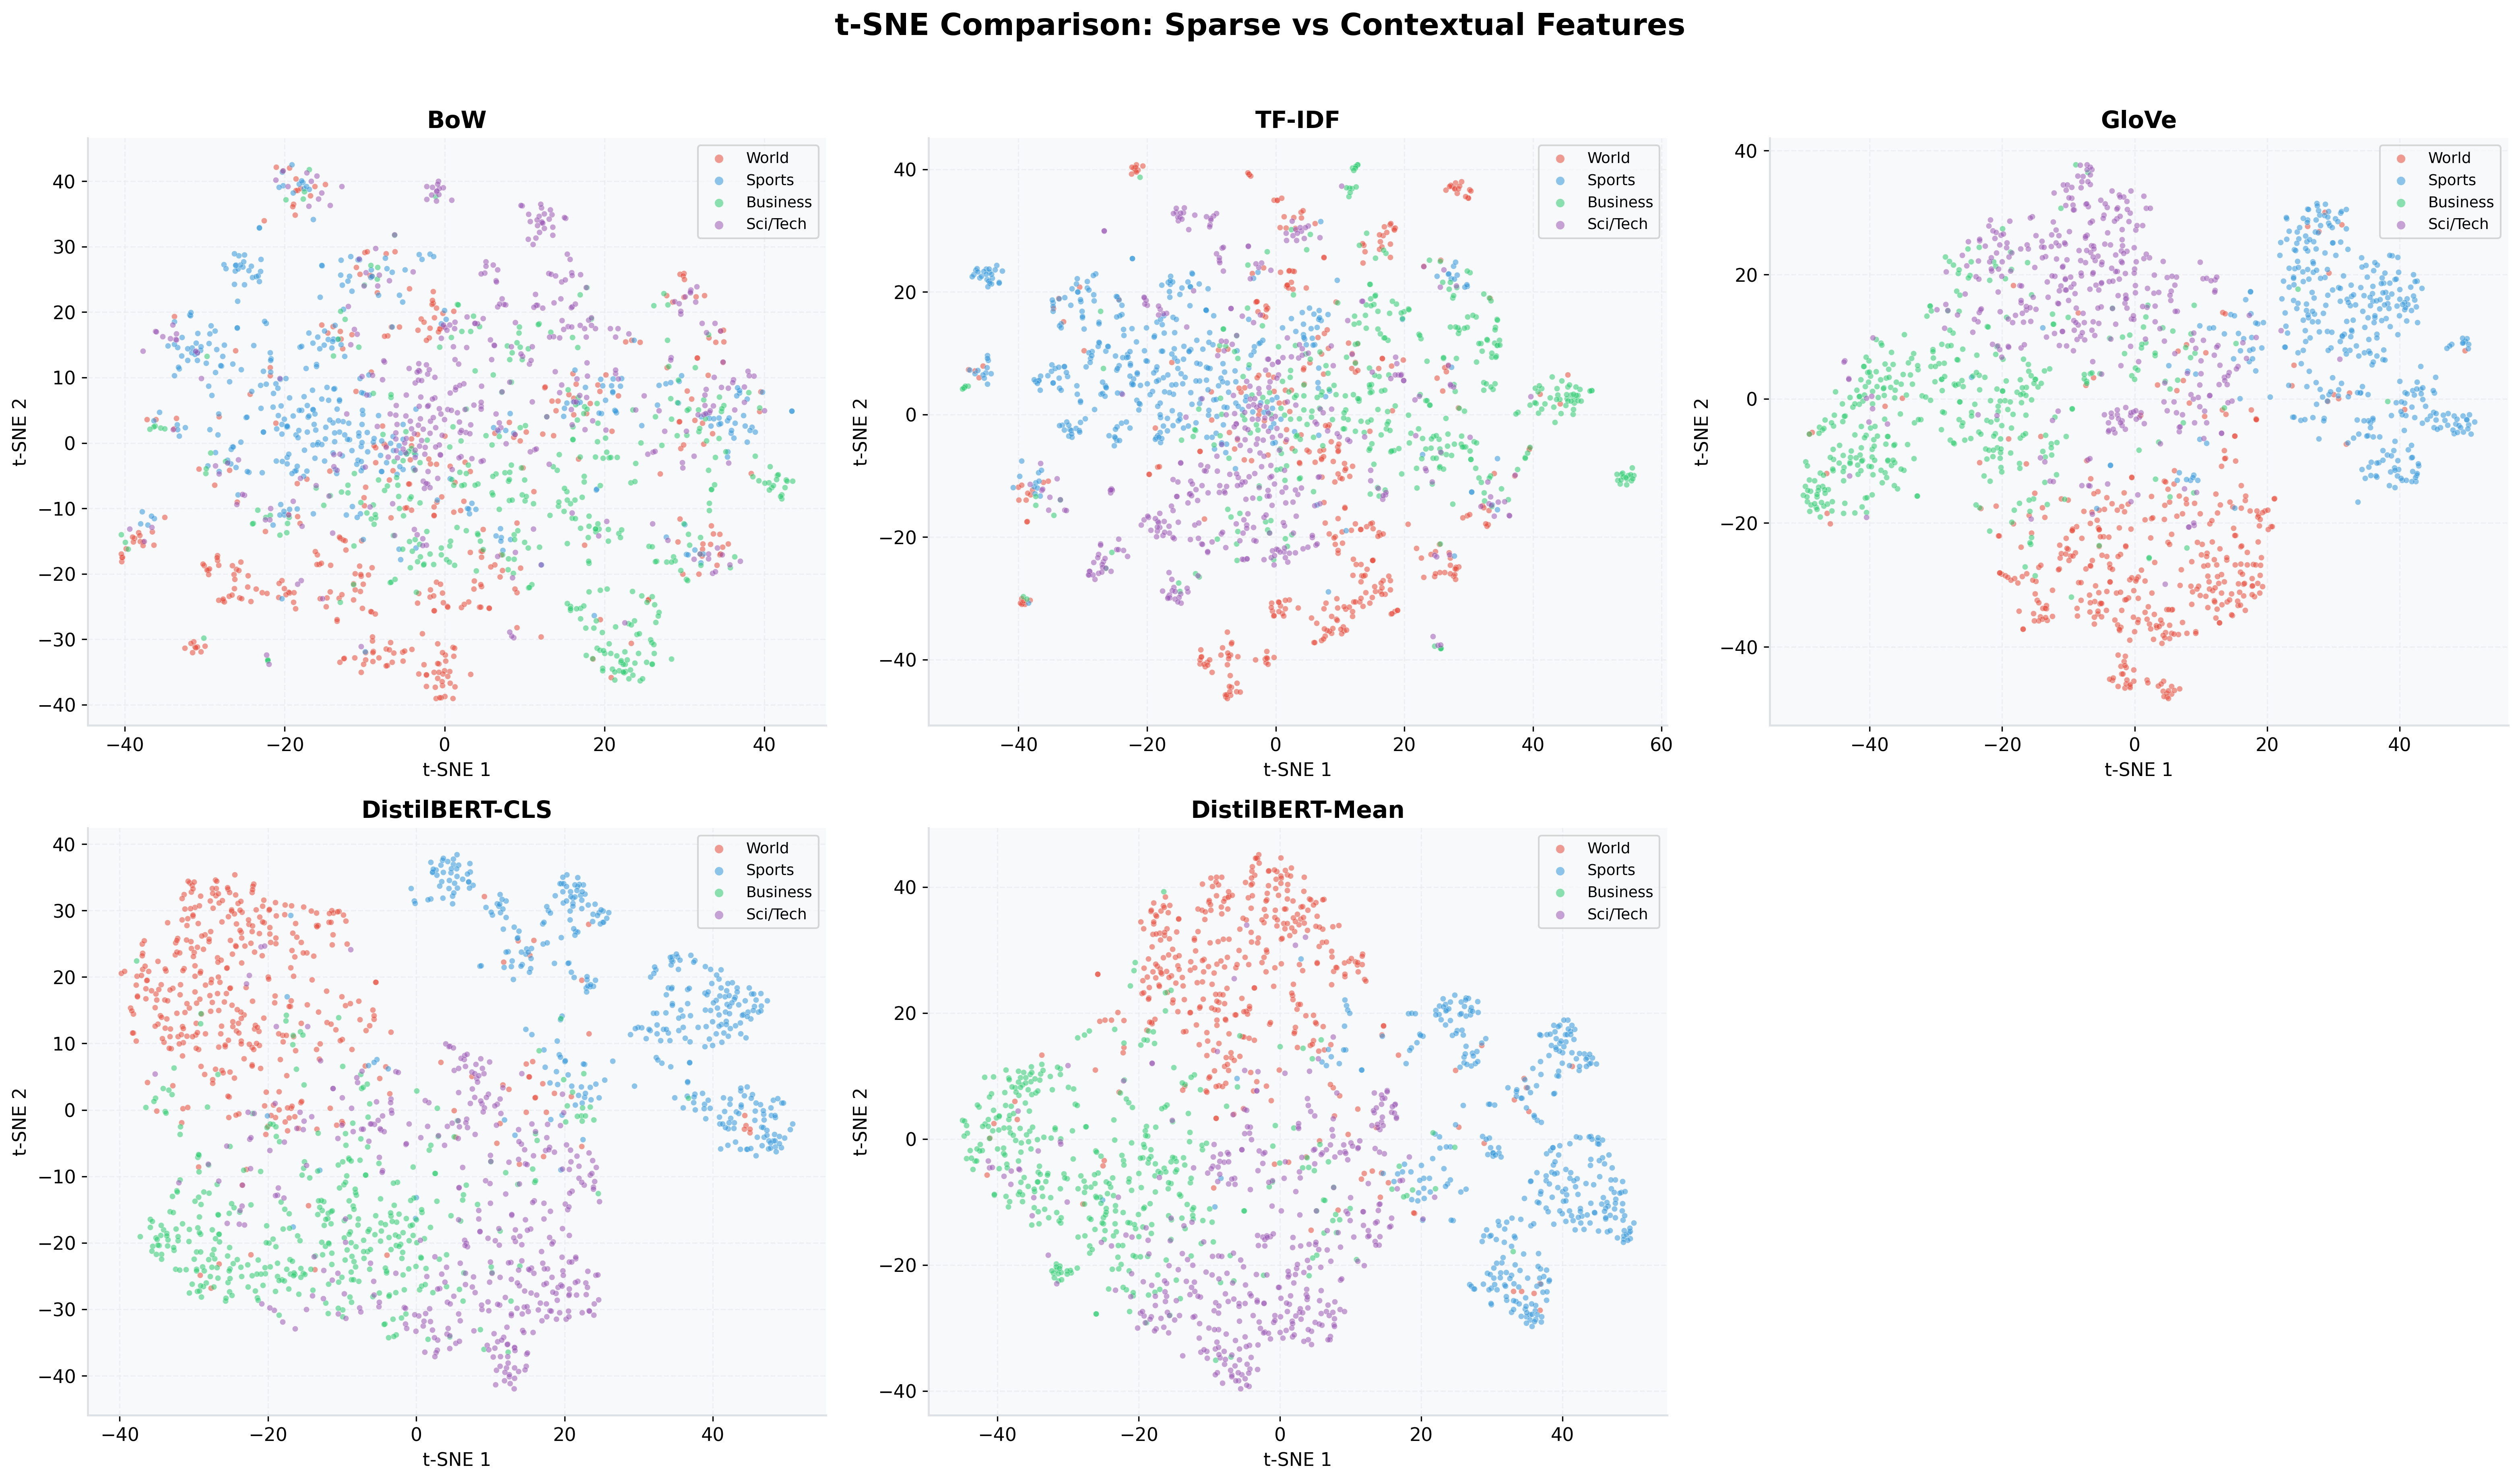
\includegraphics[width=\columnwidth]{plots/05_tsne_comparison.png}
    \caption{t-SNE projections of test-set features. DistilBERT embeddings form tighter, more separable clusters than BoW/TF-IDF.}
    \label{fig:tsne}
\end{figure}

\begin{figure}[H]
    \centering
    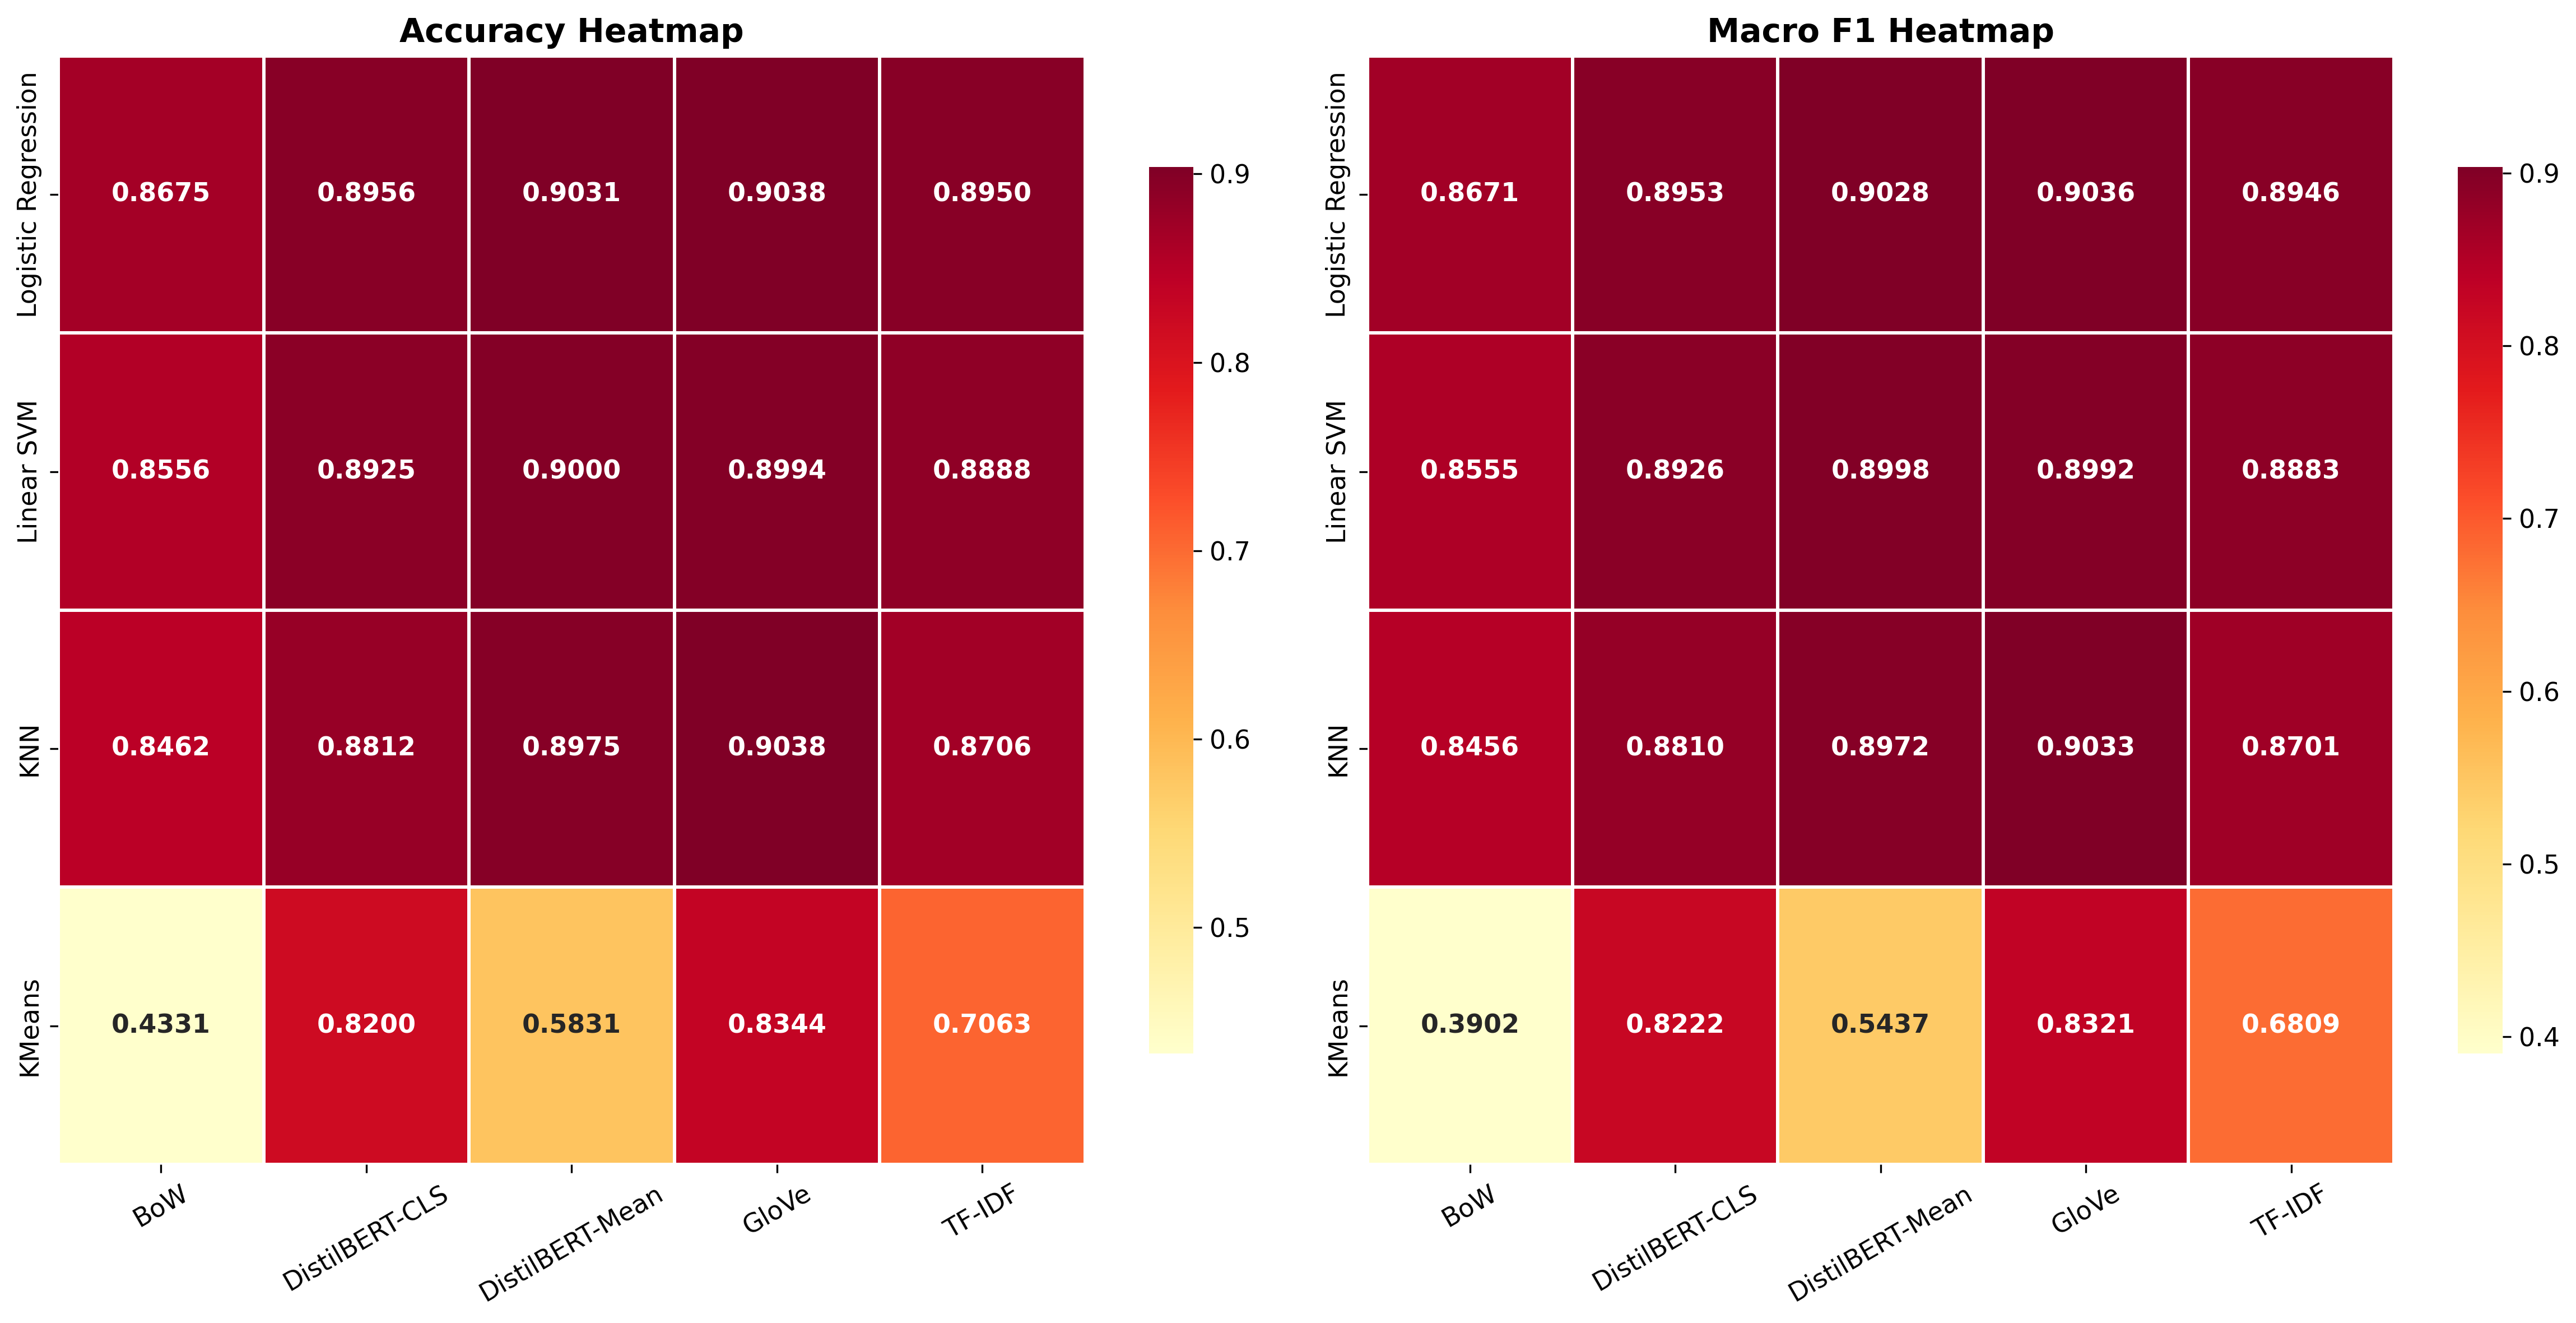
\includegraphics[width=\columnwidth]{plots/16_heatmap_results.png}
    \caption{Accuracy and Macro-F1 heatmaps across all model--feature combinations.}
    \label{fig:heatmap}
\end{figure}

\begin{figure}[H]
    \centering
    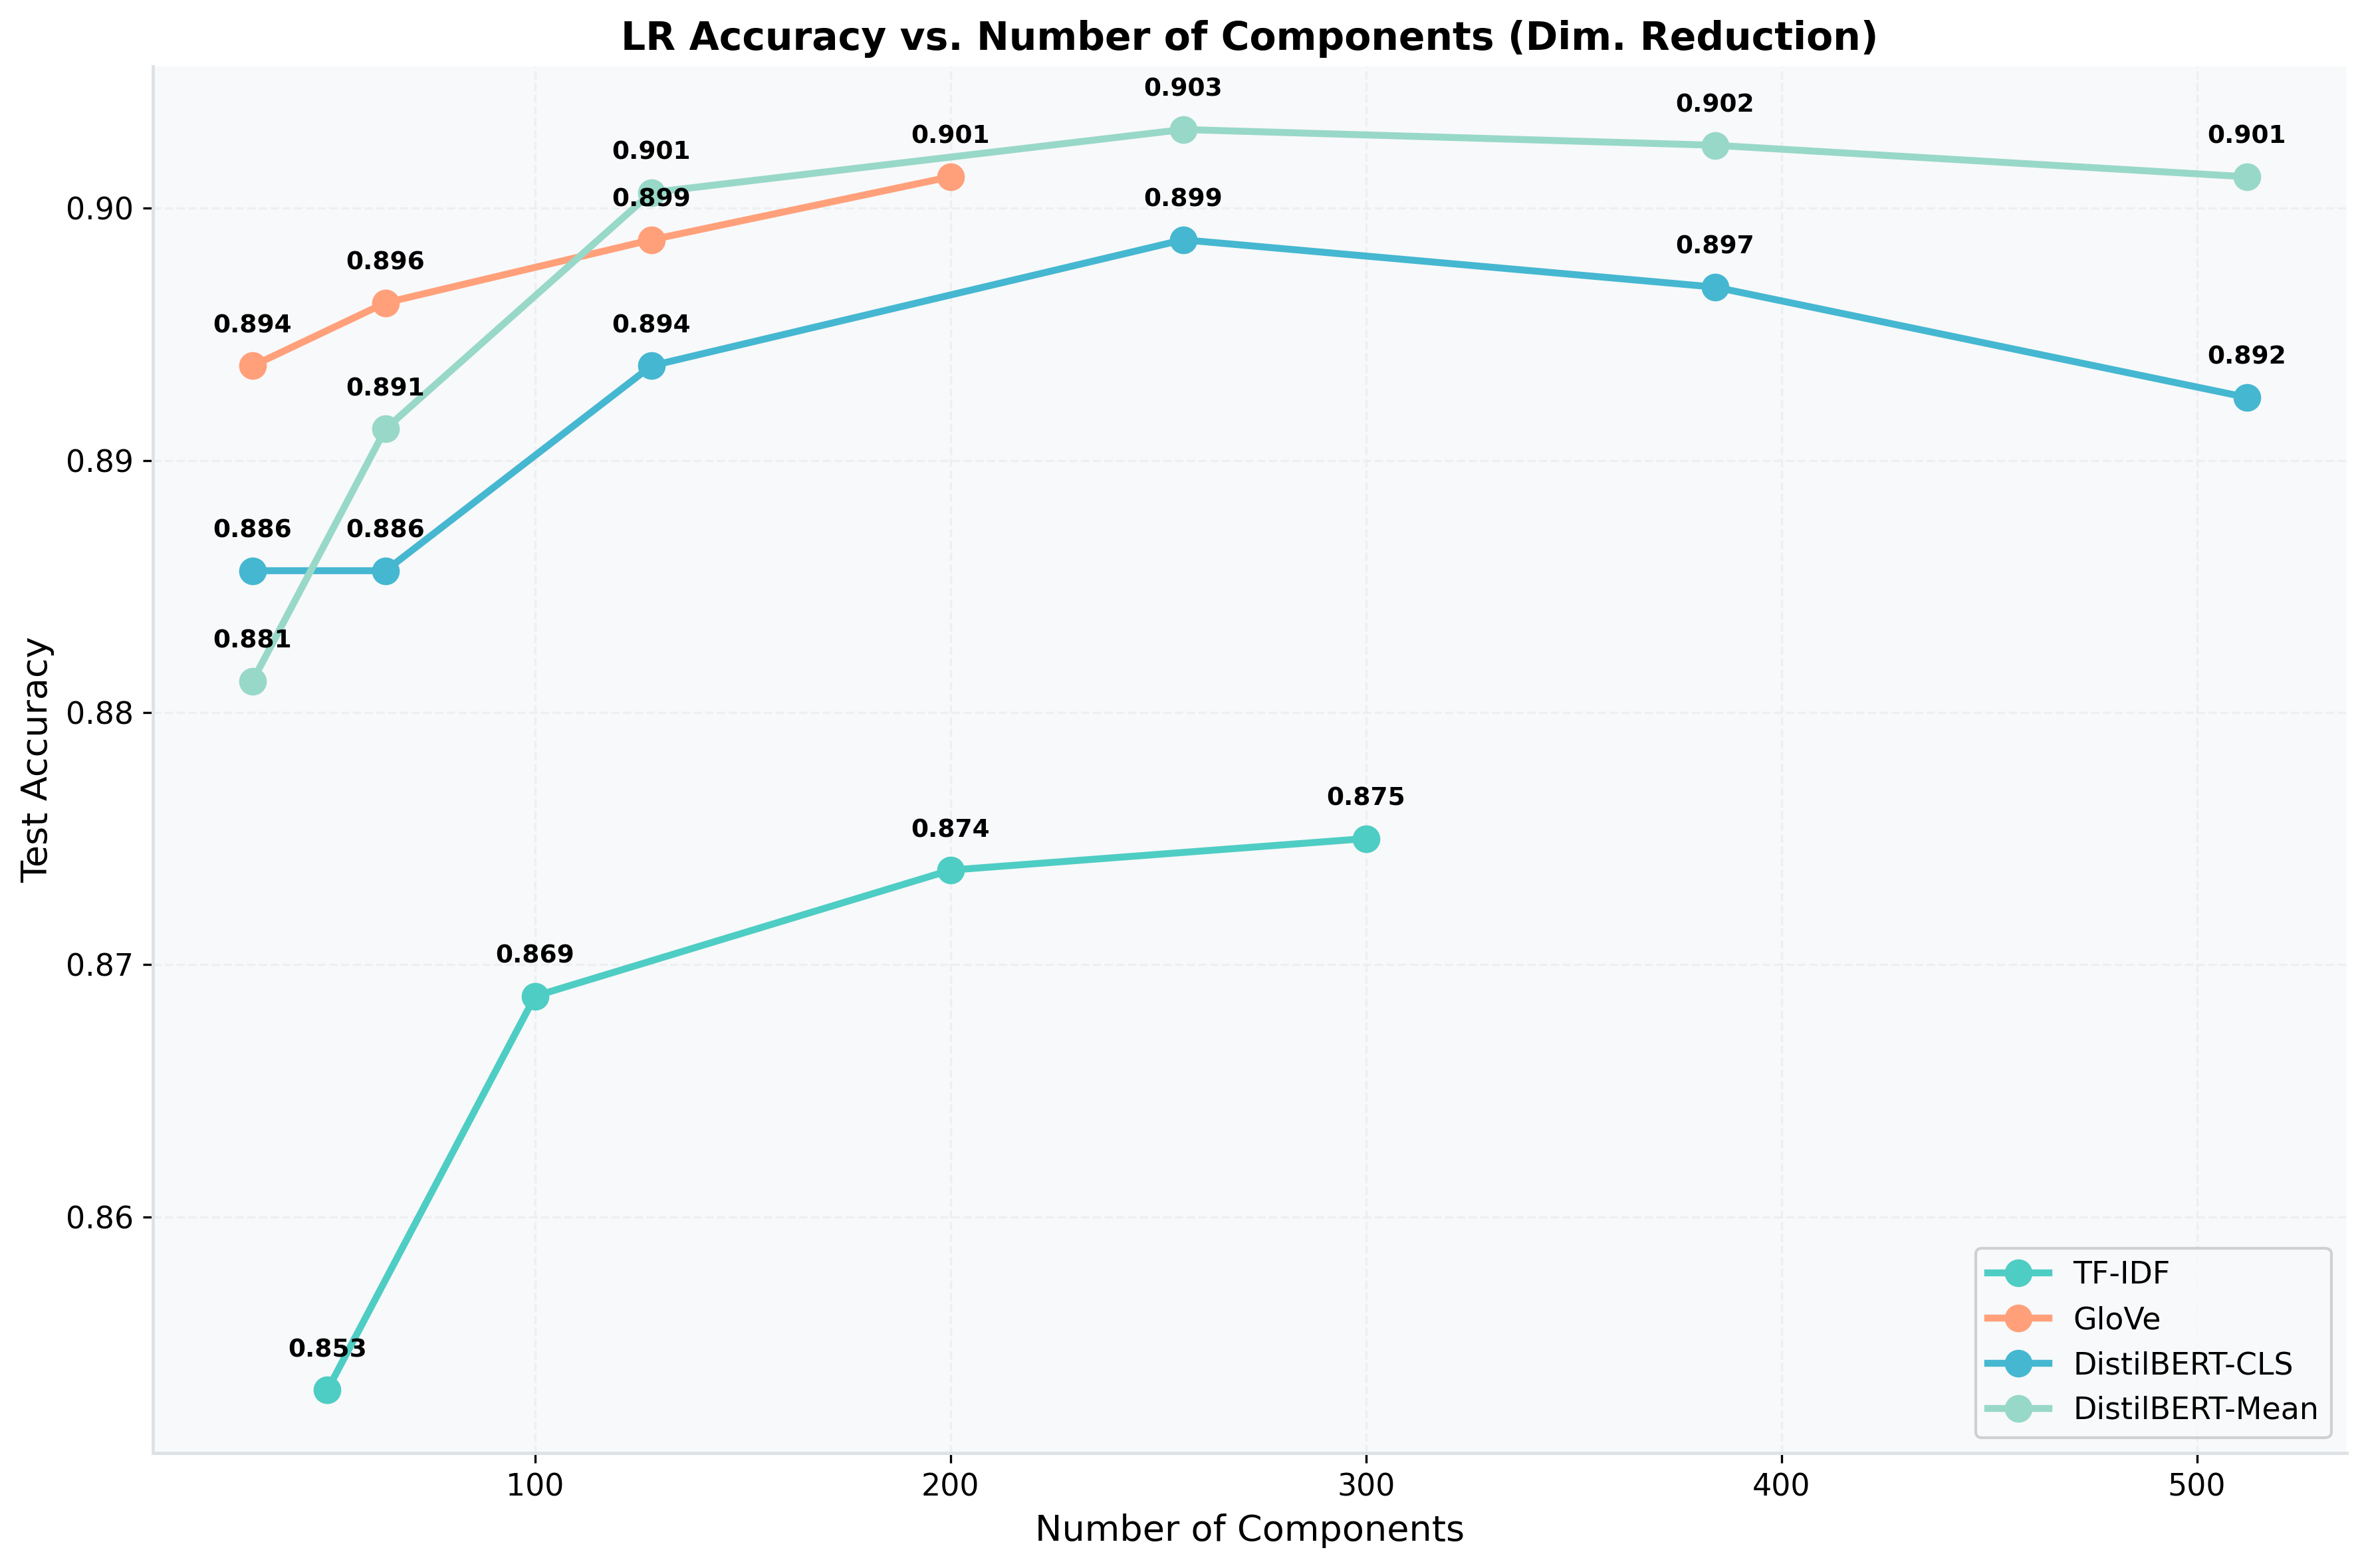
\includegraphics[width=\columnwidth]{plots/13_performance_vs_components.png}
    \caption{Classification accuracy vs.\ number of reduced dimensions.}
    \label{fig:dimred}
\end{figure}

\begin{figure}[H]
    \centering
    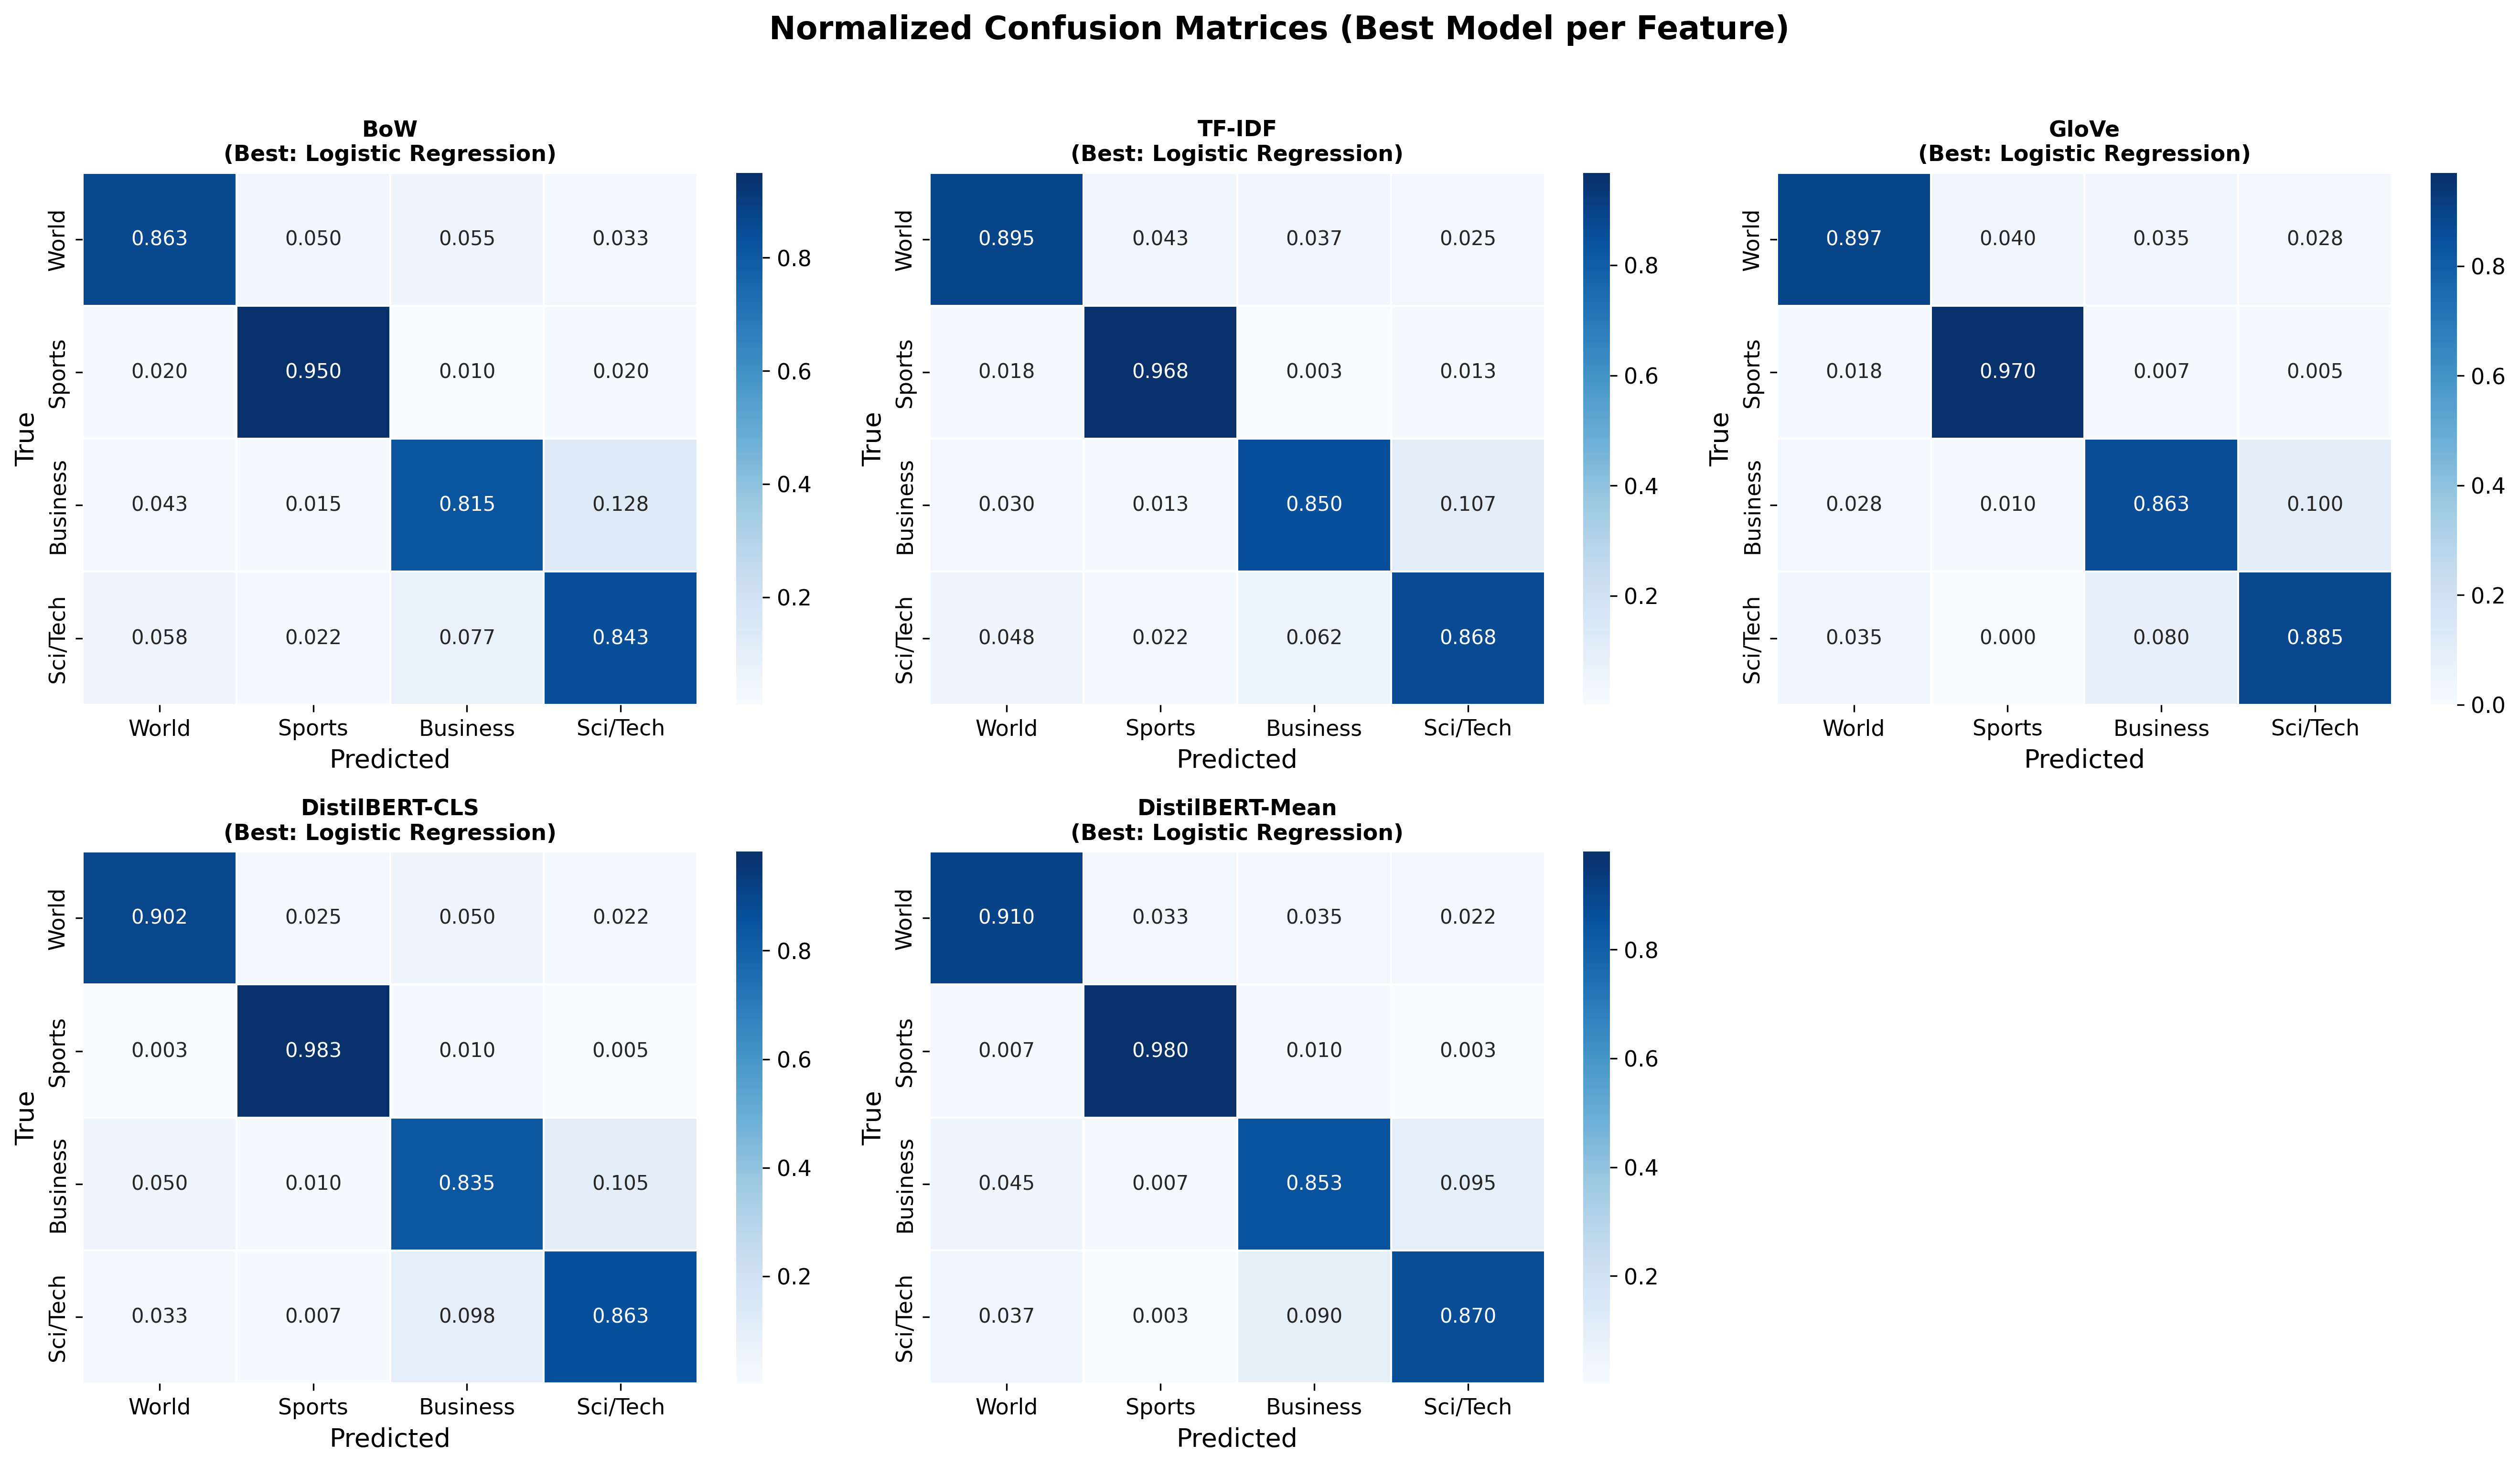
\includegraphics[width=\columnwidth]{plots/17_confusion_matrices.png}
    \caption{Normalised confusion matrices for the best model per feature type.}
    \label{fig:cm}
\end{figure}

% ============================================================
\section{Discussion}

The results confirm that contextual embeddings from pre-trained transformers encode richer semantic information than count-based sparse features, translating to higher classification accuracy on most classifiers. However, the improvement is not uniform: TF-IDF with sublinear scaling and bigrams captures enough discriminative signal for linear models to perform within a few percentage points of DistilBERT. From a practical standpoint, sparse feature extraction is lightweight while DistilBERT extraction requires GPU inference before the classical models are trained. The reported model-training time is 0.6s on sparse features vs.\ 2.7s on cached DistilBERT embeddings, excluding embedding extraction. This trade-off is crucial for deployment-constrained environments. The t-SNE plots (Figure~\ref{fig:tsne}) visually confirm that DistilBERT embeddings produce more separable clusters, explaining the higher KNN and KMeans performance on these features.

\textbf{Limitations:} Only classical ML classifiers are used; fine-tuning DistilBERT end-to-end would likely yield higher accuracy. The 8,000-sample subset may not fully represent the original AG~News distribution. KMeans assumes spherical clusters, which may not hold for all feature spaces.

% ============================================================
\section{Conclusion and Learning}

This study demonstrates that:
\begin{enumerate}[leftmargin=*,topsep=2pt,itemsep=1pt]
    \item Contextual embeddings (DistilBERT) generally outperform sparse representations when used with linear classifiers.
    \item Bigram TF-IDF remains a strong and efficient baseline, often within 1--3 percentage points of DistilBERT.
    \item KNN benefits most from dense embeddings due to the curse of dimensionality in sparse spaces.
    \item KMeans can recover meaningful topic clusters, but accuracy lags behind supervised methods by 10--20 pp.
    \item Dimensionality reduction preserves most classification signal while significantly reducing compute and memory.
\end{enumerate}

% ============================================================
\begin{thebibliography}{9}
\bibitem{agnews} X.~Zhang, J.~Zhao, and Y.~LeCun, ``Character-level convolutional networks for text classification,'' in \emph{NeurIPS}, 2015.
\bibitem{distilbert} V.~Sanh et al., ``DistilBERT, a distilled version of BERT: smaller, faster, cheaper and lighter,'' in \emph{NeurIPS Workshop}, 2019.
\bibitem{glove} J.~Pennington, R.~Socher, and C.~Manning, ``GloVe: Global vectors for word representation,'' in \emph{EMNLP}, 2014.
\bibitem{sklearn} F.~Pedregosa et al., ``Scikit-learn: Machine learning in Python,'' \emph{JMLR}, vol.~12, 2011.
\end{thebibliography}

\end{document}
